% Options for packages loaded elsewhere
\PassOptionsToPackage{unicode}{hyperref}
\PassOptionsToPackage{hyphens}{url}
\PassOptionsToPackage{dvipsnames,svgnames,x11names}{xcolor}
%
\documentclass[
  12pt,
  letterpaper,
]{article}

\usepackage{amsmath,amssymb}
\usepackage{iftex}
\ifPDFTeX
  \usepackage[T1]{fontenc}
  \usepackage[utf8]{inputenc}
  \usepackage{textcomp} % provide euro and other symbols
\else % if luatex or xetex
  \usepackage{unicode-math}
  \defaultfontfeatures{Scale=MatchLowercase}
  \defaultfontfeatures[\rmfamily]{Ligatures=TeX,Scale=1}
\fi
\usepackage{lmodern}
\ifPDFTeX\else  
    % xetex/luatex font selection
  \setmainfont[]{Baskerville}
  \setsansfont[]{Futura}
\fi
% Use upquote if available, for straight quotes in verbatim environments
\IfFileExists{upquote.sty}{\usepackage{upquote}}{}
\IfFileExists{microtype.sty}{% use microtype if available
  \usepackage[]{microtype}
  \UseMicrotypeSet[protrusion]{basicmath} % disable protrusion for tt fonts
}{}
\makeatletter
\@ifundefined{KOMAClassName}{% if non-KOMA class
  \IfFileExists{parskip.sty}{%
    \usepackage{parskip}
  }{% else
    \setlength{\parindent}{0pt}
    \setlength{\parskip}{6pt plus 2pt minus 1pt}}
}{% if KOMA class
  \KOMAoptions{parskip=half}}
\makeatother
\usepackage{xcolor}
\usepackage[margin=1in]{geometry}
\setlength{\emergencystretch}{3em} % prevent overfull lines
\setcounter{secnumdepth}{-\maxdimen} % remove section numbering


\providecommand{\tightlist}{%
  \setlength{\itemsep}{0pt}\setlength{\parskip}{0pt}}\usepackage{longtable,booktabs,array}
\usepackage{calc} % for calculating minipage widths
% Correct order of tables after \paragraph or \subparagraph
\usepackage{etoolbox}
\makeatletter
\patchcmd\longtable{\par}{\if@noskipsec\mbox{}\fi\par}{}{}
\makeatother
% Allow footnotes in longtable head/foot
\IfFileExists{footnotehyper.sty}{\usepackage{footnotehyper}}{\usepackage{footnote}}
\makesavenoteenv{longtable}
\usepackage{graphicx}
\makeatletter
\def\maxwidth{\ifdim\Gin@nat@width>\linewidth\linewidth\else\Gin@nat@width\fi}
\def\maxheight{\ifdim\Gin@nat@height>\textheight\textheight\else\Gin@nat@height\fi}
\makeatother
% Scale images if necessary, so that they will not overflow the page
% margins by default, and it is still possible to overwrite the defaults
% using explicit options in \includegraphics[width, height, ...]{}
\setkeys{Gin}{width=\maxwidth,height=\maxheight,keepaspectratio}
% Set default figure placement to htbp
\makeatletter
\def\fps@figure{htbp}
\makeatother
\newlength{\cslhangindent}
\setlength{\cslhangindent}{1.5em}
\newlength{\csllabelwidth}
\setlength{\csllabelwidth}{3em}
\newlength{\cslentryspacingunit} % times entry-spacing
\setlength{\cslentryspacingunit}{\parskip}
\newenvironment{CSLReferences}[2] % #1 hanging-ident, #2 entry spacing
 {% don't indent paragraphs
  \setlength{\parindent}{0pt}
  % turn on hanging indent if param 1 is 1
  \ifodd #1
  \let\oldpar\par
  \def\par{\hangindent=\cslhangindent\oldpar}
  \fi
  % set entry spacing
  \setlength{\parskip}{#2\cslentryspacingunit}
 }%
 {}
\usepackage{calc}
\newcommand{\CSLBlock}[1]{#1\hfill\break}
\newcommand{\CSLLeftMargin}[1]{\parbox[t]{\csllabelwidth}{#1}}
\newcommand{\CSLRightInline}[1]{\parbox[t]{\linewidth - \csllabelwidth}{#1}\break}
\newcommand{\CSLIndent}[1]{\hspace{\cslhangindent}#1}

% -----------------------
% CUSTOM PREAMBLE STUFF
% -----------------------

% -----------------
% Title block stuff
% -----------------

% Abstract
\usepackage[runin]{abstract}
\renewcommand{\abstractnamefont}{\sffamily\small\bfseries}
\renewcommand{\abstracttextfont}{\sffamily\small}
\setlength{\absleftindent}{5pt}
\setlength{\absrightindent}{\absleftindent}

% Title
\usepackage{titling}
\pretitle{\par\begin{flushleft}\LARGE\sffamily\bfseries}
\posttitle{\par\end{flushleft}\vskip 10pt}

% Keywords
\newenvironment{keywords}
{\small\sffamily{\sffamily\small\bfseries{Keywords.}}}

% Authors
\usepackage{orcidlink}  % Create automatic ORCID icons/links
%\renewcommand{\and}{\end{tabular} \hskip 3em \begin{tabular}[t]{@{\hspace{0em}}l@{}}}
\preauthor{\begin{flushleft}
           \lineskip 1.5em}
\postauthor{\end{flushleft}}

% ------------------
% Section headings
% ------------------
\usepackage{titlesec}
\titleformat*{\section}{\Large\sffamily\bfseries\raggedright}
\titleformat*{\subsection}{\large\sffamily\bfseries\raggedright}
\titleformat*{\subsubsection}{\normalsize\sffamily\bfseries\raggedright}
\titleformat*{\paragraph}{\small\sffamily\bfseries\raggedright}

%\titlespacing{<command>}{<left>}{<before-sep>}{<after-sep>}
% Starred version removes indentation in following paragraph
\titlespacing*{\section}{0em}{2em}{0.1em}
\titlespacing*{\subsection}{0em}{1.25em}{0.1em}
\titlespacing*{\subsubsection}{0em}{0.75em}{0em}

% ------------------
% Headers/Footers
% ------------------
\usepackage{fancyhdr}
\pagestyle{fancy}
\fancyhf{}
\fancyhead[L,C]{}
\fancyhead[R]{\leftmark}
\fancyfoot[L,C]{}
\fancyfoot[R]{\thepage}
\renewcommand{\headrulewidth}{1pt}
\fancypagestyle{plain}{%
    \renewcommand{\headrulewidth}{0pt}%
    \fancyhf{}%
    \fancyfoot[R]{\thepage}%
}
\renewcommand\footnoterule{\rule{\linewidth}{0.1pt}\vspace{5pt}}

% ------------------
% Captions
% ------------------
\usepackage[labelfont=bf,labelsep=period]{caption}
\captionsetup[figure]{font=footnotesize,justification=raggedright,singlelinecheck=false,format=hang}


% ---------------------------
% END CUSTOM PREAMBLE STUFF
% ---------------------------
\usepackage{float}
\usepackage{tabularray}
\usepackage[normalem]{ulem}
\usepackage{graphicx}
\UseTblrLibrary{booktabs}
\UseTblrLibrary{siunitx}
\NewTableCommand{\tinytableDefineColor}[3]{\definecolor{#1}{#2}{#3}}
\newcommand{\tinytableTabularrayUnderline}[1]{\underline{#1}}
\newcommand{\tinytableTabularrayStrikeout}[1]{\sout{#1}}
\usepackage{dcolumn}
\makeatletter
\makeatother
\makeatletter
\makeatother
\makeatletter
\@ifpackageloaded{caption}{}{\usepackage{caption}}
\AtBeginDocument{%
\ifdefined\contentsname
  \renewcommand*\contentsname{Table of contents}
\else
  \newcommand\contentsname{Table of contents}
\fi
\ifdefined\listfigurename
  \renewcommand*\listfigurename{List of Figures}
\else
  \newcommand\listfigurename{List of Figures}
\fi
\ifdefined\listtablename
  \renewcommand*\listtablename{List of Tables}
\else
  \newcommand\listtablename{List of Tables}
\fi
\ifdefined\figurename
  \renewcommand*\figurename{Figure}
\else
  \newcommand\figurename{Figure}
\fi
\ifdefined\tablename
  \renewcommand*\tablename{Table}
\else
  \newcommand\tablename{Table}
\fi
}
\@ifpackageloaded{float}{}{\usepackage{float}}
\floatstyle{ruled}
\@ifundefined{c@chapter}{\newfloat{codelisting}{h}{lop}}{\newfloat{codelisting}{h}{lop}[chapter]}
\floatname{codelisting}{Listing}
\newcommand*\listoflistings{\listof{codelisting}{List of Listings}}
\makeatother
\makeatletter
\@ifpackageloaded{caption}{}{\usepackage{caption}}
\@ifpackageloaded{subcaption}{}{\usepackage{subcaption}}
\makeatother
\makeatletter
\@ifpackageloaded{tcolorbox}{}{\usepackage[skins,breakable]{tcolorbox}}
\makeatother
\makeatletter
\@ifundefined{shadecolor}{\definecolor{shadecolor}{rgb}{.97, .97, .97}}
\makeatother
\makeatletter
\makeatother
\makeatletter
\makeatother
\ifLuaTeX
  \usepackage{selnolig}  % disable illegal ligatures
\fi
\IfFileExists{bookmark.sty}{\usepackage{bookmark}}{\usepackage{hyperref}}
\IfFileExists{xurl.sty}{\usepackage{xurl}}{} % add URL line breaks if available
\urlstyle{same} % disable monospaced font for URLs
\hypersetup{
  pdftitle={Navigating Ancestry and Racial Classification Amongst Multiracial Indigenous American},
  pdfauthor={Matthew Guerra},
  pdfkeywords={Indigenous identity, multiracial
studies, ancestry, racial decision-making, racial
classification, settler-colonialism, QuantCrit, American Community
Survey},
  colorlinks=true,
  linkcolor={blue},
  filecolor={Maroon},
  citecolor={Blue},
  urlcolor={red},
  pdfcreator={LaTeX via pandoc}}


\title{Navigating Ancestry and Racial Classification Amongst Multiracial
Indigenous American\thanks{Thanks to everyone for checking this out.}}
% subtitles do not seem to work with article class?
%%\subtitle{}

\author{
{\bfseries \normalsize Matthew Guerra~\orcidlink{0009-0003-2658-442X}}%
\thanks{Corresponding author.} \\%
 \small University of Oregon, Sociology \\%
{\footnotesize \url{mguerra2@uoregon.edu}} \\\vspace{10pt}
}

\predate{}
\postdate{}
\date{}
\begin{document}

% for some reason this does not work in header
\renewcommand{\abstractname}{Abstract.}

\fancyhead[L]{Navigating Ancestry and Racial Classification}

% need to redefine this environment to get enough spacing of 
% bibliography after title
\renewenvironment{CSLReferences}[2] % #1 hanging-ident, #2 entry spacing
 {% don't indent paragraphs
  \vspace{10pt}
  \setlength{\parindent}{0pt}
  % turn on hanging indent if param 1 is 1
  \ifodd #1
  \let\oldpar\par
  \def\par{\hangindent=\cslhangindent\oldpar}
  \fi
  % set entry spacing
  \setlength{\parskip}{#2\cslentryspacingunit}
 }%
 {}

\maketitle
%\noindent \rule{\linewidth}{.5pt}
\begin{abstract}
Current research on race and multiracial individuals recognizes that
Indigenous racial identity is fluid and often contested. Using a
settler-colonial theoretical framework and the recommendations of
QuantCrit literature, this research project expands understanding of
multi-racial Indigenous identity and demonstrates how ancestry
influences racial ``decision-making'' for Indigenous Americans. By
leveraging data from the American Community Survey (ACS) from 2010 to
2020, the relationship between an individuals reported ancestry and
their self-identified racial classification is investigated by
estimating multinomial logistic regression models. The results indicate
the relationship between various predictorss, and a persons likelihood
to identify as Indigenous alone, multi-racial, or to distance themself
from their Indigenous ancestry and identity in favor of their other
racial identity. When these findings are evaluated within the context of
settler-colonialism, many previously confounding findings can be linked
to the social reality that respondents navigate as Indigenous Americans.
\end{abstract}
\begin{keywords}
\def\sep{;\ }
Indigenous identity\sep multiracial studies\sep ancestry\sep racial
decision-making\sep racial
classification\sep settler-colonialism\sep QuantCrit\sep 
American Community Survey
\end{keywords}
%\noindent \rule{\linewidth}{.5pt}
\ifdefined\Shaded\renewenvironment{Shaded}{\begin{tcolorbox}[boxrule=0pt, frame hidden, interior hidden, enhanced, sharp corners, borderline west={3pt}{0pt}{shadecolor}, breakable]}{\end{tcolorbox}}\fi

\hypertarget{introduction}{%
\section{Introduction}\label{introduction}}

Who is Indigenous and who is not? Where do multiracial Indigenous
Americans fit in this equation? One group of scholars has attempted to
better understand Indigenous identity by asking similar questions by
determining which factors are associated with strong Indigenous
identity, how this identity is contested and understood at an
interpersonal and community level, and how the Indigenous population has
grown over time {[}Liebler (2010) Lucero (2014) McKay (2021). Indigenous
identity becomes even more complicated when considering multiracial
Indigenous Americans, which has led to additional research in this area,
although limited. Articles on Indigenous identity generally cover the
racial decision-making process for multiracial Indigenous people in the
United States, since many Indigenous people have mixed racial
ancestries. This social reality requires Indigenous American respondents
to make conscious decisions when listing their race. In the case of
multiracial Indigenous people their known racial ancestry either
conflicts with or affirms their answer, and they must reconcile with
that decision. Understanding this decision-making process is crucial for
gaining insights into contemporary shifts in racial boundary formation
and the individual considerations that shape racial identification for
Indigenous Americans.

However, in 2020 Dwanna L. McKay, Kirsten Vinyeta, and Kari M. Norgaard
published an article titled ``Theorizing Race and Settler Colonialism
within U.S. Sociology'' which calls for a critical approach to how race
is studied within Sociology, particularly how the focus on assimilation
fails to confront its violent and often deadly nature of assimilation
for Indigenous Americans under settler colonialism. Their article
established that as researchers and academics, we are complicit in the
erasure of Indigenous people, and the continued reification of harmful
narratives can only be stopped by engaging with settler colonialism
theory when conducting our research.

These considerations led to the theoretical engagement explored later in
this paper to prepare for a critical and nuanced approach to
quantitative research has often been critiqued for its inability to
speak to individual experiences, and for those who study race, there
have been critiques of using race as a static category that does not
reflect the social reality of race as a social construct, which
parallels the arguments mentioned above about settler colonialism within
the sociology of race and ethnicity. This dynamic nature of race means
that it can and does change, and is influenced by various social factors
and processes at both the micro and macro level which is why a critical
approach to the interpretation and contextualization of results from
quantitative research is imperative to furthering understanding without
sacrificing reflexivity Zuberi \& Bonilla-Silva (2008).

\hypertarget{theoretical-framework}{%
\section{Theoretical Framework}\label{theoretical-framework}}

In 2018 the Journal of Race Ethnicity and Education published a special
issue titled ``QuantCrit: Rectifying Quantitative Methods Through
Critical Race Theory'', where various scholars critically engaged with
quantitative research and methods, using CRT to determine whether
quantitative research is capable of being used to further a critical
race agenda in education research and beyond Garcia, López, \& Vélez
(2018). This approach is not new, however, and has already been
established in Du Bosian sociology, most notably in Du Bois's The
Philadelphia Negro. The Philadelphia Negro has been described as a great
example of an alternate approach to quantitative research that can be
liberating and work to counter oppressive racial narratives while
presenting statistical analysis alongside theoretical arguments Conwell
\& Loughran (2023). Du Bois's approach came from necessity due to the
popularity of theories like Social Darwinism which placed Black people
at the bottom of the hierarchy, a reality that required the questioning
of assumptions and working against the grain of how quantitative
research was and often continues to be done. In this article, this
approach will be replicated as best as possible, and part of that
requires delving into settler colonial theory and current research
related to Indigenous identity in the U.S. to create a historical and
theoretical context that this paper will rely on.

In his article ``Settler Colonialism and the Elimination of the
Native,'' Patrick Wolfe describes what he coins the `logic of
elimination' (2006). This logic explains the operation of colonizers
arriving and settling on lands already inhabited by another group,
specifically that settler colonialism requires the implementation of
violence to achieve the goals of a settler society and replace
Indigenous structures with those of the settler society. The replacement
of Indigenous structures ultimately included the removal and
dispossession of Indigenous people themself, which was justified through
the racialization of Indigenous people A. A. Gonzales \& Kertész (2023).
Additionally, since the structures of racialization and
settler-colonialism inform each other, an analysis of racial
decision-making would be incomplete without considering how Indigenous
racial formation came to be in the US.

For Indigenous Americans, membership within a tribe is often a key part
of this process to distinguish between those who are Indigenous and
those who are not. This concept is demonstrated in research done to
identify what barriers to tribal enrollment exist for individuals who
have been separated from their family and community via adoption and the
foster system Landers, Danes, Morgan, Merritt, \& White Hawk (2021). It
was identified that tribal enrollment was key for these individuals to
establish and prove their own identity and seek collective identity
within the tribe. Essentially, tribal enrollment exists as a ``process
of mutual verification between the individual and the tribe''
(p.~1374).~ Additionally, the forceful removal of Indigenous children
from their families between the 1800s and 1970s by the United States
federal government---via relocation, boarding schools, child welfare
removal, adoption era practices, and so on, has created a group of
Indigenous Americans, and their descendants, who have been removed from
their family and culture thus further causing turmoil in how they
conceptualize their identity. The Federal Acknowledgement Project of
1978, furthered this process since it created an administrative process
that required any group wishing to be acknowledged by the federal
government as a legitimate tribe to meet certain criteria established by
the federal government, further establishing Indigenous American
identity as an administrative process rather than of racial, ethnic, or
cultural identity A. Gonzales, Kertész, \& Tayac (2007).

Blood quantum often exists as a requirement for tribal membership
through a blood quantum minimum which functions as a benchmark of
authenticity for who is recognized as Native American by the U.S.
government and continues to endure as a key feature of Indigenous
identity Rodriguez-Lonebear (2021). This system was established as
criteria for federal recognition in response to laws like Virginia's
Racial Integrity Act of 1924 and the Indian Reorganization Act (IRA) of
1934 which helped establish racial divisions and criteria on how to
quantify Native American identity, respectively A. Gonzales et al.
(2007). This establishes that determining Native American identity
functions as an administrative process rather than a cultural process of
a distinct racial and ethnic group, allowing a governing body to
determine who can self-identify a certain way Lambert (2019).

\begin{itemize}
\item
  his would be considered important to talk about engaging with for
  example when thinking about homelands, ie looking at connections to
  land
\item
  should look at churning race and think about how part of the goal of
  settler colonialism is the replacement of Indigenous people by
  settlers to become indigenous in their place as a potential
  explanation? Especially when thinking about hypodescent and why this
  decision-making process might be occurringIt is key to note that
  findings made in this paper are not intended to dispute but rather
  support the findings found in other projects both qualitative and
  quantitative and base them on the lived reality these studies reflect

  Furthermore, the interpretation of results through the lens of CRT,
  QuantCrit, or settler-colonialism may not be able to account for every
  finding however engaging with the social reality Indigenous Americans
  navigate only serves to expand and explain current understandings
  regarding Indigenous identity, particularly multi-racial Indigenous
  identity

  This call for more critically engaged quantitative research is at the
  basis of this article, meaning that the results will have been
  interpreted within the context of CRT as well as settler-colonialism
  due to its focus on Indigenous people.~Methods and data
\end{itemize}

\hypertarget{sample-selection-and-data}{%
\subsection{Sample Selection and Data}\label{sample-selection-and-data}}

The data used for this project was compiled from the American Community
Survey data for the years 2010 - 2020. I seek to analyze the race
reporting of individuals who indicate Indigenous ancestry in addition to
White, Black, or Asian ancestry. For this study, the term Indigenous is
used in place of the American Indian and Alaskan Native (AIAN) terms as
it is generally more accepted and has grown in popularity in current
literature when discussing identity. The sample did not include
individuals who listed their race as Latino or Pacific Islander.Part of
the data organization of this project required the identification of a
multiracial population, specifically an Indigenous multiracial
population. To accomplish this goal the Goldstein and Morning method was
adopted, which relies on looking at adults' self-reported ancestry,
which in turn does not rely on the question of racial identity and
instead allows for the construction of a multiracial population based on
respondents' self-reported racial ancestry. In regards to the sample,
this means looking at respondents who listed Indigenous ancestry in
addition to a racially distinct racial ancestry other than
Indigenous.Once this group was identified further case selection was
performed as these results were compared to their race response. When
looking at their racial ancestry and race response, respondents were
divided into 4 distinct categories:1) Indigenous alone, which contained
respondents that listed their race solely as Indigenous 2) Consistent
which included respondents that acknowledged their racial ancestry in
full by selecting a racial option that reflected that ancestry 3)
Non-Indigenous Race alone, where respondents did acknowledge their
Indigenous ancestry when selecting their race response and 4)
Inconsistent, where respondents race response did not reflect their
racial ancestry in any capacity

Outcome variable: race response Predictor variables: metro, homeland,
education above high school, gender and hispanicity These ancestry
responses were compared to what their race response and divided into the
following groups: Indigenous alone, Multiracial, and Other Race alone
where Indigenous alone consisted of those respondents who identified a
mixed-ancestry of Indigenous plus one other racial ancestry yet listed
their race response as Indigenous alone. Multiracial was those
respondents who identified their mixed--Indigenous ancestry and listed a
multiracial race response. Other race alone consisted of those
respondents with a mixed-Indigenous racial ancestry but listed their
racial response as the other race (ie. ancestry listed as Indigenous and
Asian but list race as Asian only).

\hypertarget{methods}{%
\subsection{Methods}\label{methods}}

The analysis was conducted through creation of several multinomial logit
models, which predict the likelihood of a respondent to identify as
either Indigenous alone, Multiracial, or other race alone. Three sets of
models were created, each set had a different reference category:
``Indigenous/White'', ``Indigenous/Black'', and ``Indigenous/Asian''

\begin{figure}[!t]

{\centering 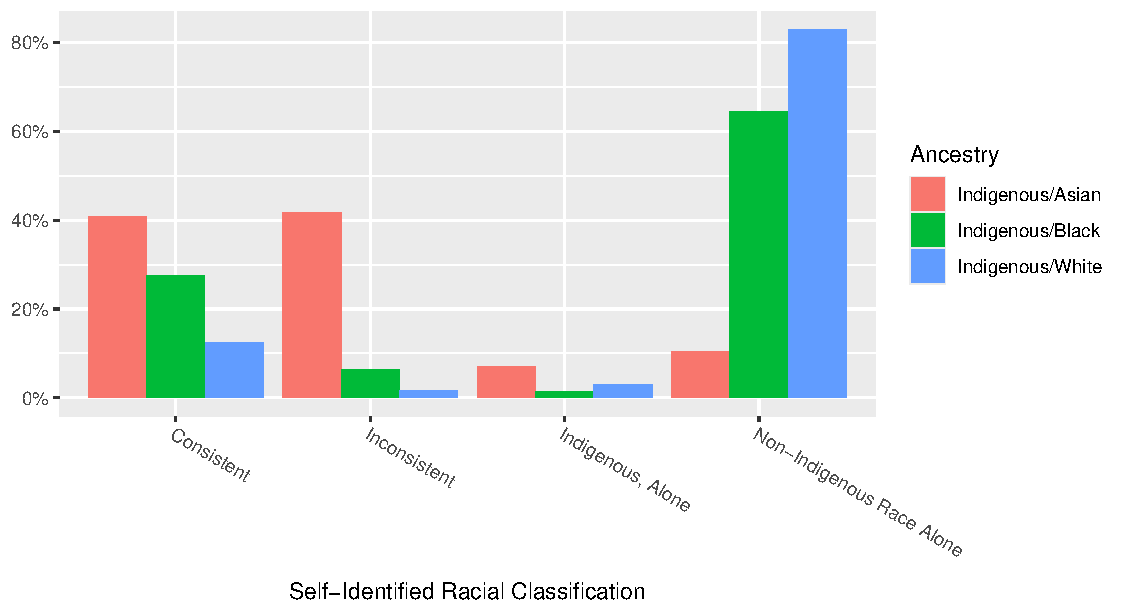
\includegraphics{main_manuscript_files/figure-pdf/fig-race-ancestry-1.pdf}

}

\caption{\label{fig-race-ancestry}Comparing listed ancestry and race
classification}

\end{figure}

\hypertarget{weights-16-9-variable}{%
\section{weights: 16 (9 variable)}\label{weights-16-9-variable}}

initial value 599314.460436 iter 10 value 284800.079668 iter 20 value
256524.479851 iter 30 value 254381.017785 final value 254010.499668
converged \# weights: 20 (12 variable) initial value 599314.460436 iter
10 value 333726.839486 iter 20 value 270019.984945 iter 30 value
249315.133813 iter 40 value 249023.098803 final value 249022.958481
converged \# weights: 44 (30 variable) initial value 599314.460436 iter
10 value 253458.711343 iter 20 value 252519.732821 iter 30 value
247515.058087 iter 40 value 245369.541898 iter 40 value 245369.540313
iter 40 value 245369.540302 final value 245369.540302 converged :::
\{.cell-output-display\}

\hypertarget{tbl-white-indigenous}{}
\begin{table}
\caption{\label{tbl-white-indigenous}White/Indigenous Models }\tabularnewline

\centering
\begin{talltblr}[         %% tabularray outer open
entry=none,label=none,
note{}={+ p < 0.1, * p < 0.05, ** p < 0.01, *** p < 0.001},
]                     %% tabularray outer close
{                     %% tabularray inner open
colspec={Q[]Q[]Q[]Q[]Q[]Q[]Q[]Q[]Q[]Q[]},
cell{1}{2}={c=3,}{halign=c,},
cell{1}{5}={c=3,}{halign=c,},
cell{1}{8}={c=3,}{halign=c,},
column{1}={halign=l,},
column{2}={halign=c,},
column{3}={halign=c,},
column{4}={halign=c,},
column{5}={halign=c,},
column{6}={halign=c,},
column{7}={halign=c,},
column{8}={halign=c,},
column{9}={halign=c,},
column{10}={halign=c,},
row{1}={halign=c,},
hline{23}={1,2,3,4,5,6,7,8,9,10}{solid, 0.05em, black},
}                     %% tabularray inner close
\toprule
& (1) &  &  & (2) &  &  & (3) &  &  \\ \cmidrule[lr]{2-4}\cmidrule[lr]{5-7}\cmidrule[lr]{8-10}
& Inconsistent & Indigenous, Alone & Non-Indigenous Race Alone & Inconsistent & Indigenous, Alone & Non-Indigenous Race Alone & Inconsistent & Indigenous, Alone & Non-Indigenous Race Alone \\ \midrule %% TinyTableHeader
(Intercept)        & \num{-2.577}*** & \num{-1.171}*** & \num{1.992}***  & \num{-2.263}*** & \num{-1.541}*** & \num{2.304}***  & \num{-1.888}*** & \num{-1.687}*** & \num{2.562}***  \\
& (\num{0.038})   & (\num{0.021})   & (\num{0.011})   & (\num{0.040})   & (\num{0.024})   & (\num{0.012})   & (\num{0.066})   & (\num{0.048})   & (\num{0.023})   \\
MetroCMetropolitan & \num{0.711}***  & \num{-0.356}*** & \num{-0.158}*** & \num{0.518}***  & \num{-0.160}*** & \num{-0.349}*** & \num{0.469}***  & \num{-0.172}*** & \num{-0.297}*** \\
& (\num{0.041})   & (\num{0.025})   & (\num{0.012})   & (\num{0.042})   & (\num{0.025})   & (\num{0.013})   & (\num{0.042})   & (\num{0.026})   & (\num{0.013})   \\
MetroCUnknown      & \num{0.111}*    & \num{-0.096}*** & \num{-0.032}*   & \num{0.057}     & \num{-0.049}+   & \num{-0.085}*** & \num{0.056}     & \num{-0.044}    & \num{-0.080}*** \\
& (\num{0.051})   & (\num{0.029})   & (\num{0.015})   & (\num{0.051})   & (\num{0.029})   & (\num{0.015})   & (\num{0.051})   & (\num{0.029})   & (\num{0.015})   \\
HomelandPYes       &                  &                  &                  & \num{-0.809}*** & \num{0.653}***  & \num{-0.799}*** & \num{-0.795}*** & \num{0.654}***  & \num{-0.799}*** \\
&                  &                  &                  & (\num{0.037})   & (\num{0.021})   & (\num{0.011})   & (\num{0.037})   & (\num{0.021})   & (\num{0.011})   \\
EducAHS Diploma    &                  &                  &                  &                  &                  &                  & \num{-0.058}    & \num{0.033}     & \num{0.084}***  \\
&                  &                  &                  &                  &                  &                  & (\num{0.044})   & (\num{0.034})   & (\num{0.016})   \\
EducASome College  &                  &                  &                  &                  &                  &                  & \num{-0.118}**  & \num{0.103}**   & \num{-0.174}*** \\
&                  &                  &                  &                  &                  &                  & (\num{0.042})   & (\num{0.032})   & (\num{0.015})   \\
EducACollege       &                  &                  &                  &                  &                  &                  & \num{-0.393}*** & \num{0.046}     & \num{-0.329}*** \\
&                  &                  &                  &                  &                  &                  & (\num{0.048})   & (\num{0.036})   & (\num{0.017})   \\
GenderMan          &                  &                  &                  &                  &                  &                  & \num{-0.306}*** & \num{0.004}     & \num{-0.255}*** \\
&                  &                  &                  &                  &                  &                  & (\num{0.026})   & (\num{0.019})   & (\num{0.009})   \\
HispanicHispanic   &                  &                  &                  &                  &                  &                  & \num{1.526}***  & \num{0.641}***  & \num{-1.494}*** \\
&                  &                  &                  &                  &                  &                  & (\num{0.046})   & (\num{0.049})   & (\num{0.034})   \\
Age                &                  &                  &                  &                  &                  &                  & \num{-0.003}*** & \num{0.001}*    & \num{-0.001}*** \\
&                  &                  &                  &                  &                  &                  & (\num{0.001})   & (\num{0.001})   & (\num{0.000})   \\
Num.Obs.           & \num{432314}    &                  &                  & \num{432314}    &                  &                  & \num{432314}    &                  &                  \\
R2                 & \num{0.002}     &                  &                  & \num{0.022}     &                  &                  & \num{0.036}     &                  &                  \\
R2 Adj.            & \num{0.002}     &                  &                  & \num{0.022}     &                  &                  & \num{0.036}     &                  &                  \\
AIC                & \num{508039.0}  &                  &                  & \num{498069.9}  &                  &                  & \num{490799.1}  &                  &                  \\
BIC                & \num{508137.8}  &                  &                  & \num{498201.6}  &                  &                  & \num{491128.4}  &                  &                  \\
RMSE               & \num{0.27}      &                  &                  & \num{0.27}      &                  &                  & \num{0.27}      &                  &                  \\
\bottomrule
\end{talltblr}
\end{table}

:::

\hypertarget{results}{%
\section{Results}\label{results}}

In

\hypertarget{conclusion}{%
\section{Conclusion}\label{conclusion}}

\hypertarget{bibliography}{%
\section*{References}\label{bibliography}}
\addcontentsline{toc}{section}{References}

\hypertarget{refs}{}
\begin{CSLReferences}{1}{0}
\leavevmode\vadjust pre{\hypertarget{ref-conwell_quantitative_2023}{}}%
Conwell, J. A., \& Loughran, K. (2023). Quantitative {Inquiry} in the
{Early} {Sociology} of {W}. {E}. {B}. {Du} {Bois}. \emph{Du Bois Review:
Social Science Research on Race}, 1--23.
\url{https://doi.org/10.1017/S1742058X23000206}

\leavevmode\vadjust pre{\hypertarget{ref-garcia_quantcrit_2018}{}}%
Garcia, N. M., López, N., \& Vélez, V. N. (2018). {QuantCrit}:
Rectifying quantitative methods through critical race theory. \emph{Race
Ethnicity and Education}, \emph{21}(2), 149--157.
\url{https://doi.org/10.1080/13613324.2017.1377675}

\leavevmode\vadjust pre{\hypertarget{ref-gonzales_colonialism_2023}{}}%
Gonzales, A. A., \& Kertész, J. (2023). Colonialism and the
{Racialization} of {Indigenous} {Identity}. In M. Walter, T. Kukutai, A.
A. Gonzales, \& R. Henry (Eds.), \emph{The {Oxford} {Handbook} of
{Indigenous} {Sociology}} (p. 0). Oxford University Press.
\url{https://doi.org/10.1093/oxfordhb/9780197528778.013.36}

\leavevmode\vadjust pre{\hypertarget{ref-gonzales_eugenics_2007}{}}%
Gonzales, A., Kertész, J., \& Tayac, G. (2007). Eugenics as {Indian}
{Removal}: {Sociohistorical} {Processes} and the {De}(con)struction of
{American} {Indians} in the {Southeast}. \emph{The Public Historian},
\emph{29}(3), 53--67. \url{https://doi.org/10.1525/tph.2007.29.3.53}

\leavevmode\vadjust pre{\hypertarget{ref-lambert2019}{}}%
Lambert. (2019). How grandma kate lost her cherokee blood and what this
says about race, blood, and belonging in indian country. \emph{American
Indian Quarterly}, \emph{43}(2), 135.
\url{https://doi.org/10.5250/amerindiquar.43.2.0135}

\leavevmode\vadjust pre{\hypertarget{ref-landers2021}{}}%
Landers, A. L., Danes, S. M., Morgan, A. A., Merritt, S., \& White Hawk,
S. (2021). My relatives are waiting: Barriers to tribal enrollment of
fostered/adopted American Indians. \emph{Journal of Marriage and
Family}, \emph{83}(5), 1373--1400.
\url{https://doi.org/10.1111/jomf.12797}

\leavevmode\vadjust pre{\hypertarget{ref-liebler_homelands_2010}{}}%
Liebler, C. A. (2010). Homelands and indigenous identities in a
multiracial era. \emph{Social Science Research}, \emph{39}(4), 596--609.
\url{https://doi.org/10.1016/j.ssresearch.2010.02.003}

\leavevmode\vadjust pre{\hypertarget{ref-lucero_its_2014}{}}%
Lucero, N. M. (2014). {``{It}'s not about place, it's about what's
inside''}: {American} {Indian} women negotiating cultural connectedness
and identity in urban spaces. \emph{Women's Studies International
Forum}, \emph{42}, 9--18.
\url{https://doi.org/10.1016/j.wsif.2013.10.012}

\leavevmode\vadjust pre{\hypertarget{ref-mckay_real_2021}{}}%
McKay, D. L. (2021). Real {Indians}: {Policing} or {Protecting}
{Authentic} {Indigenous} {Identity}? \emph{Sociology of Race and
Ethnicity}, \emph{7}(1), 12--25.
\url{https://doi.org/10.1177/2332649218821450}

\leavevmode\vadjust pre{\hypertarget{ref-rodriguez-lonebear_blood_2021}{}}%
Rodriguez-Lonebear, D. (2021). The {Blood} {Line}: {Racialized}
{Boundary} {Making} and {Citizenship} among {Native} {Nations}.
\emph{Sociology of Race and Ethnicity}, \emph{7}(4), 527--542.
\url{https://doi.org/10.1177/2332649220981589}

\leavevmode\vadjust pre{\hypertarget{ref-zuberi_white_2008}{}}%
Zuberi, T., \& Bonilla-Silva, E. (Eds.). (2008). \emph{White logic,
white methods: Racism and methodology}. Lanham: Rowman \& Littlefield
Publishers.

\end{CSLReferences}



\end{document}
